GlueX, short for the Gluonic Excitation experiment located at the Thomas Jefferson National Accelerator Facility (JLab), first began collecting publication-quality data in 2016 with the goal of establishing the spectrum of light mesonic states including hybrid mesons and glueballs.

\begin{figure}
  \begin{center}
    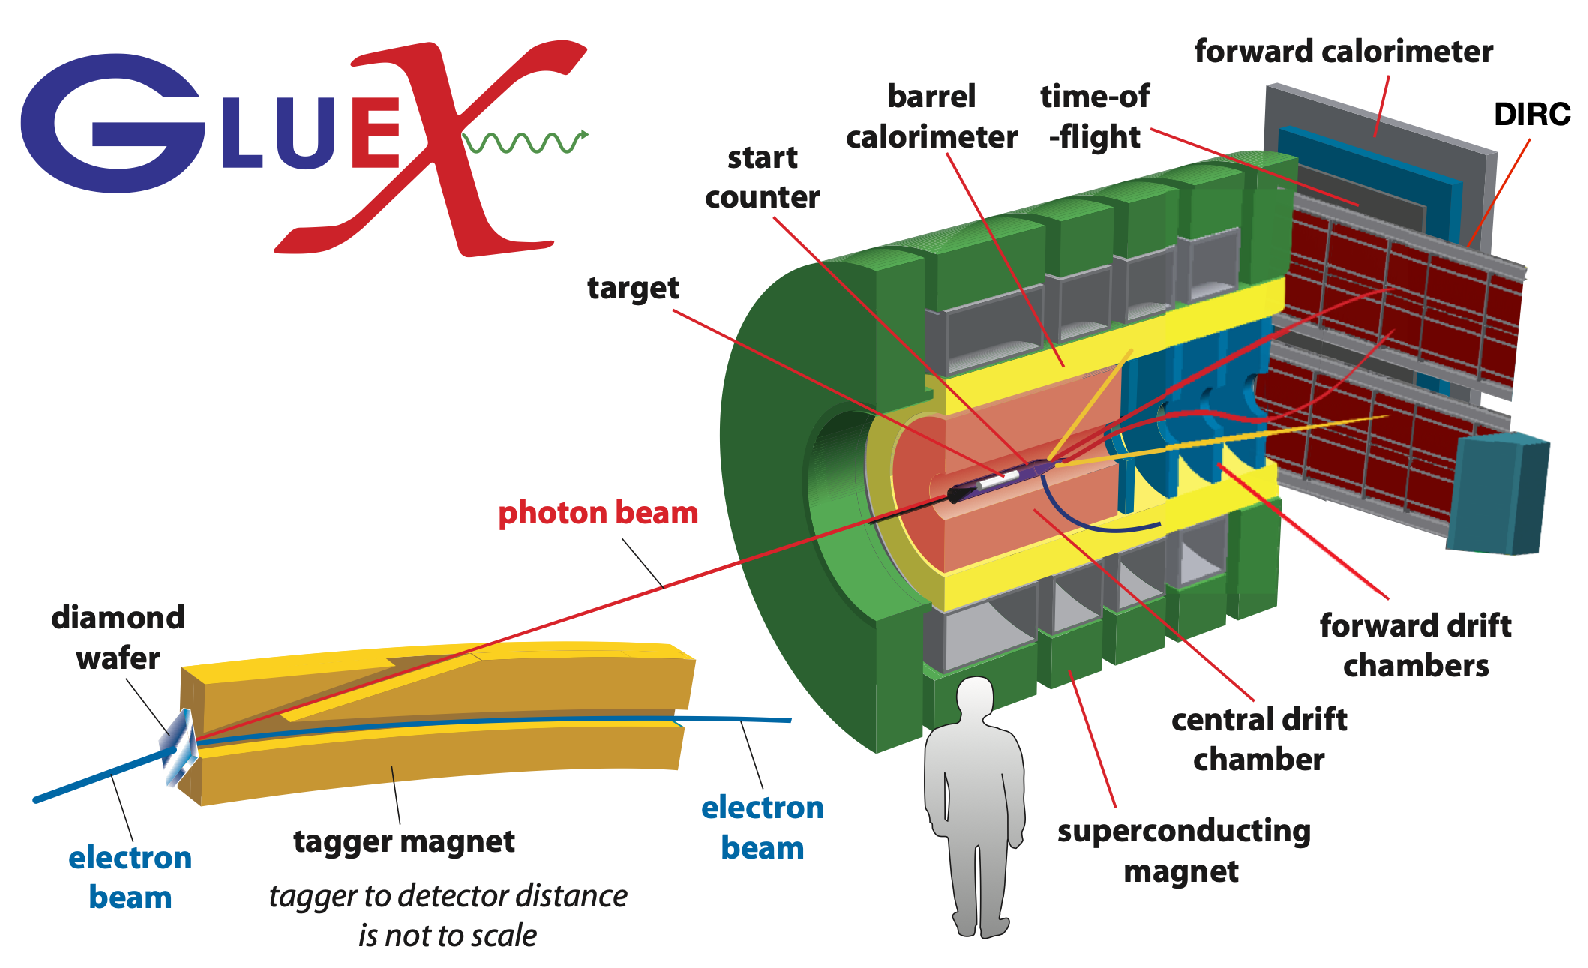
\includegraphics[width=0.8\textwidth]{figures/gluex_detector.png}
  \end{center}
  \caption{A diagram of the GlueX detector at JLab. The DIRC detector was installed in 2019 and was only present for about half of the data analyzed in this study.{\color{red}CITE}}\label{fig:gluex-detector}
\end{figure}

GlueX receives an unpolarized electron beam from the Continuous Electron Beam Accelerator Facility (CEBAF), which is then converted to linearly polarized photons via coherent bremsstrahlung from a diamond radiator (see \Cref{fig:gluex-detector}). The scattering electrons are detected in an array of high-resolution scintillators called the Tagger Microscope (TAGM) which covers beam energies between $8$ and $\SI{9}{\giga\eV}$, a region of energy referred to as the ``coherent peak''. The orientation of the diamond radiator is optimized to produce the highest photon polarization and flux in this region (see \Cref{fig:gluex-polarization}). The rest of the energy range, regions from about $3$--$\SI{8}{\giga\eV}$ and $9$--$\SI{12}{\giga\eV}$, are covered by the lower-resolution Tagger Hodoscope (TAGH). These elements are used to determine only the photon energy, which is equal to the difference between the incident and outgoing electron energies~\cite{adhikari_gluex_2021}.


\begin{figure}
  \begin{center}
    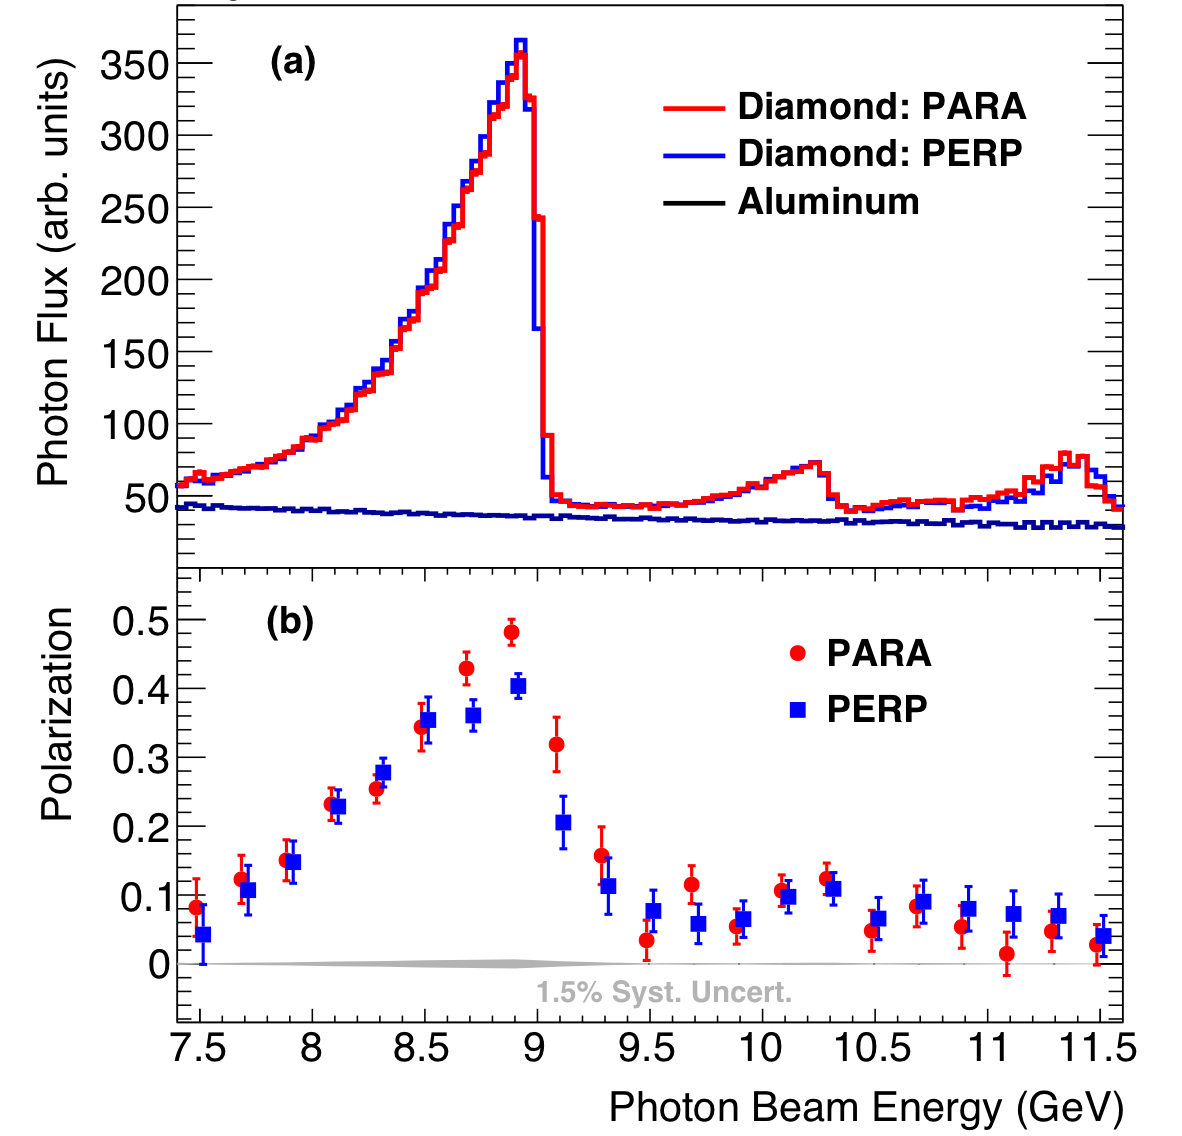
\includegraphics[width=0.95\textwidth]{figures/gluex_polarization.png}
  \end{center}
  \caption{(a) Collimated photon beam intensity versus energy as measured by the Pair Spectrometer. (b) Collimated photon beam polarization as a function of beam energy, as measured by the Triplet Polarimeter, with data points offset horizontally by $\pm\SI{0.015}{\giga\eV}$ for clarity. The labels PARA and PERP refer to orientations of the diamond radiator that result in polarization planes that are parallel and perpendicular to the horizontal, respectively (figure and caption from \cite{adhikari_gluex_2021}).}\label{fig:gluex-polarization}
\end{figure}


\begin{figure}
  \begin{center}
    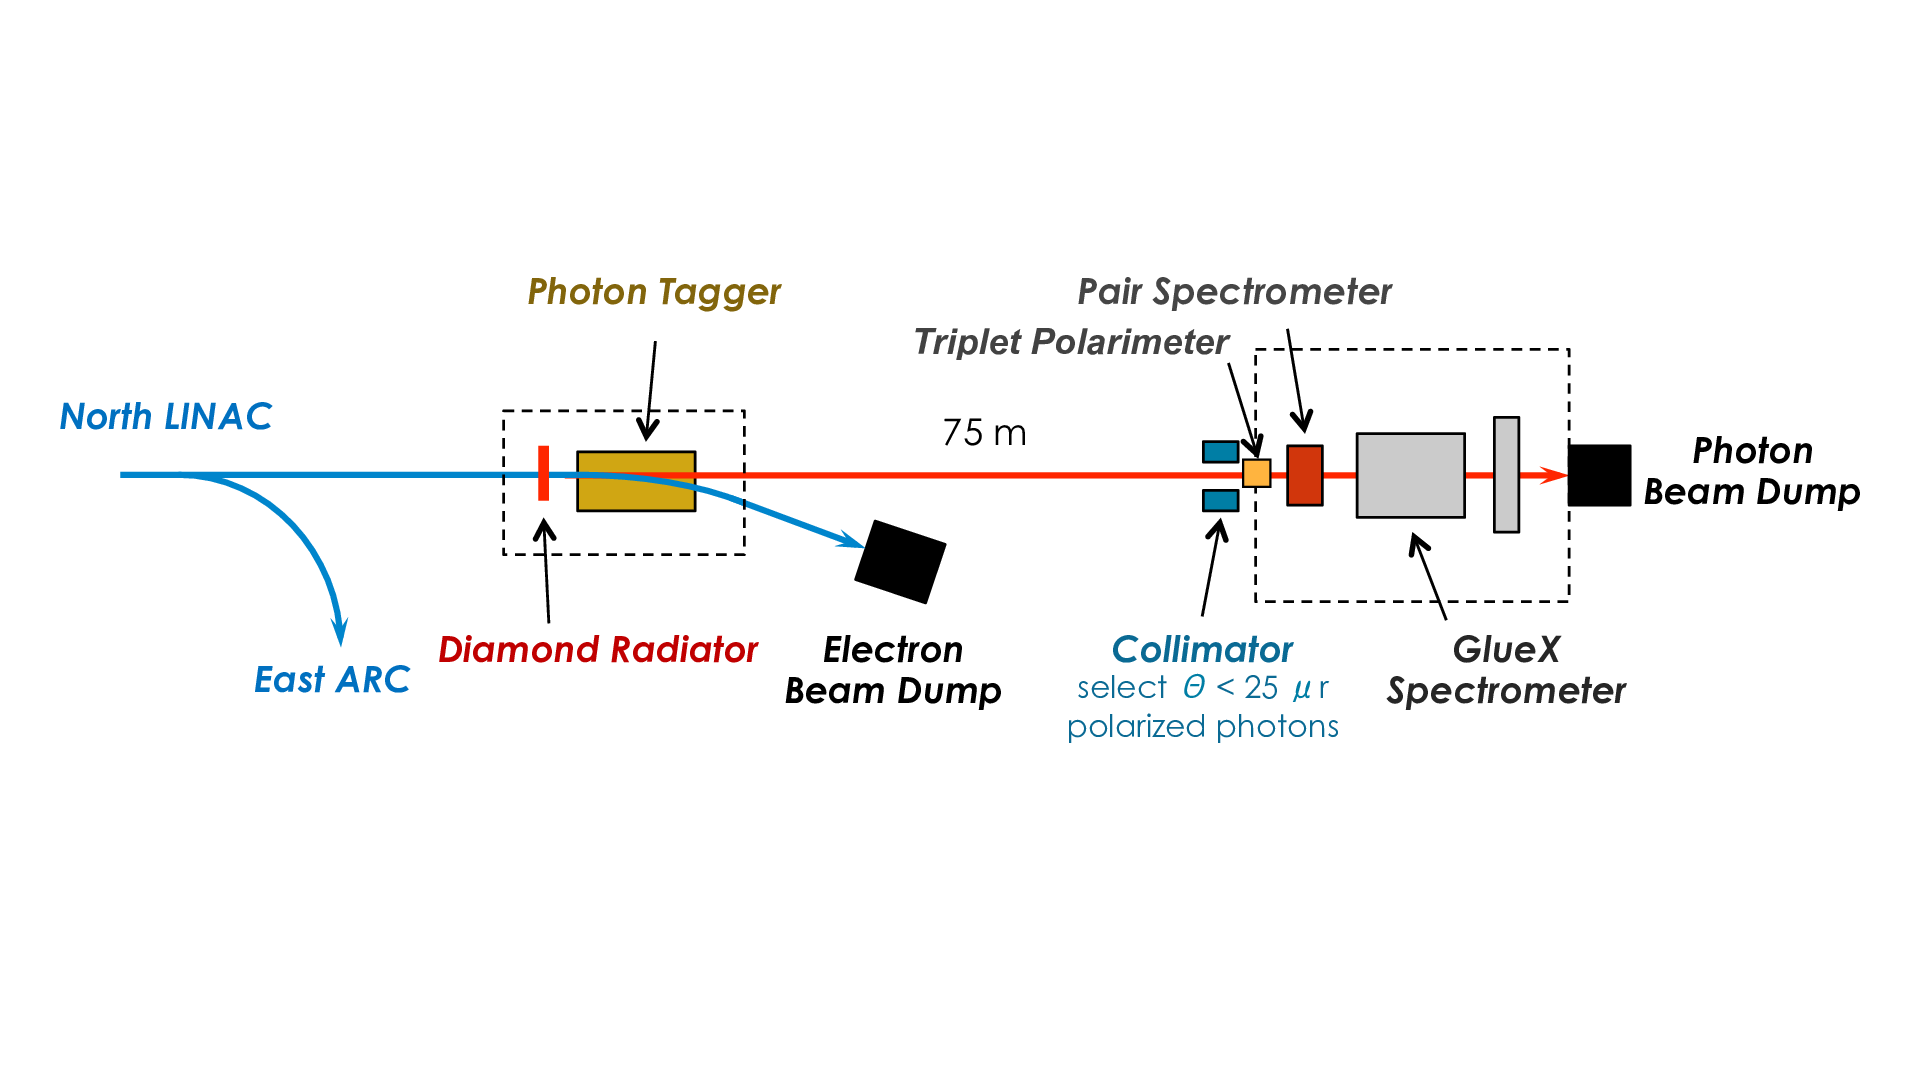
\includegraphics[width=0.95\textwidth]{figures/gluex_beamline.png}
  \end{center}
  \caption{A diagram of the beamline layout of the Triplet Polarimeter (TPOL) and Pair Spectrometer (PS) used to measure the polarization and beam flux.}\label{fig:gluex-beamline}
\end{figure}


To measure the polarization properties of the photon beam as well as the photon flux, the photon beam passes through a thin beryllium foil which induces $e^+e^-$ pair production on some known fraction of the photons (see \Cref{fig:gluex-beamline}). The angular distribution of the produced electrons along with an electron knocked out of the foil medium as part of the pair production process is measured by the Triplet Polarimeter (TPOL) to determine the photon polarization fraction. The Pair Spectrometer (PS) then counts the pair-produced electrons in coincidence with the TAGM and TAGH detectors. A known fraction\footnote{We know the radiation length of the beryllium foil, and this along with the radiator thickness determines the fraction of photons which will pass through without interacting.} of the beam is converted to $e^+e^-$ pairs in this way, allowing for an accurate measurement of the photon flux and the energy dependence of the polarization fraction.

Photons which do not pair-produce in the beryllium radiator interact with a liquid hydrogen cryotarget, which maintains a temperature of $\SI{20.1}{\K}$, allowing the contents to act as a stationary proton target. A set of thin scintillators called the Start Counter (ST) surrounds the target, which captures the initial signals (and azimuthal angles) from reaction products and associates them with the electron radio frequency (RF) beam bunch from which the reaction originated\footnote{The electron beam bunches from the CEBAF arrive every $\SI{4}{\nano\s}$, a rate of $\SI{250}{\mega\hertz}$.}. Any products of the reaction next pass through either the Central Drift Chamber (CDC) or Forward Drift Chamber (FDC) depending on their trajectory (particles within $1^{\circ}$\textendash$10^{\circ}$ of the beamline pass through the FDC, and the detector has partial coverage up to $20^{\circ}$). The CDC is filled with long metal tubes at various orientations, while the FDC chambers are flat disks. Each tube/disk is filled with a gaseous mixture of argon and carbon dioxide\footnote{These particular gases and the mixture ratio are chosen to reduce interfering effects from the magnetic field of the main solenoid.} with a thin wire running through their center of each tube and an array of wires crossing the plane of each disk. The wire and tube/disk faces are held at a voltage differential, and charged particles passing through the chambers ionize the gases inside. The faster-moving electrons move towards the positively charged wires, while the slower-moving ions move towards the tubes/disks. The combination of these signals allows for the reconstruction of the trajectories of each charged particle which passes through each chamber. Both detectors are situated inside a solenoid with a magnetic field around $\SI{2}{\tesla}$, and this field bends the trajectories of charged particles, allowing for proper identification of the sign of the charge as well as the particle's momentum.

The Barrel Calorimeter (BCAL) surrounding the CDC and the Forward Calorimeter (FCAL) in front of the FDC measure the energy of electromagnetic deposits from interactions with charged and neutral particles. This includes photons originating from the decays of light neutral mesons like the $\pi^0$ and $\eta$. Because such neutral particles pass through the CDC and FDC without detection, these calorimeters are necessary for their reconstruction. However, since there are no intermediate trajectories, GlueX is unable to reconstruct the decay vertices of these neutral particles. Since we are studying a reaction with a fully charged final state, this might not seem important. However, in {\color{red}Section ?}, we will discuss the study of neutral decays of $K_S^0\to 2\pi^0 \to 4\gamma$, where the reconstruction will be severely limited due to the inability to reconstruct the decay vertex of the $K_S^0$.

There is a final scintillator array called the Time-of-Flight (TOF) detector situated immediately between the FDC and the FCAL. In combination with the ST and the RF timing information from the accelerator, this aids in charged-particle identification via a measurement of the flight time between the two detectors. Additionally, in 2019, an additional detector, the DIRC\footnote{An acronym for Detection of Internally Reflected Cherenkov light} detector was installed between the TOF and FDC to further aid in identification of charged pions and kaons. This detector measures the angle of the cone of Cherenkov radiation emitted by relativistic charged particles, which can be used to ascertain their velocity via the relation $\cos\theta_c \sim 1/v$. When compared to measurements of the particle's momentum, this detector can be used to distinguish pions, kaons, and protons. Further information about the GlueX detector and the DIRC can be found in references \cite{adhikari_gluex_2021} and \cite{ali_installation_2020} respectively.

The data analyzed in this thesis were collected in four separate ``run periods'' across two experiment ``phases'', denoted Phase-I and Phase-II. Phase-I consists of three run periods, notated Spring 2017, Spring 2018, and Fall 2018 by the season and year when data collection began, and Phase-II contains one run period, Spring 2020\footnote{This run technically began at the end of 2019} and is the only dataset which was collected after the DIRC installation. The total luminosity, coherent peak range, and luminosity in the coherent peak for each run period is listed in \Cref{tab:run-info}.


\begin{table}
  \begin{center}
    \begin{tabular}{ccccc}\toprule
      Experiment & Run Period & Luminosity ($E_\gamma > \SI{6.0}{\giga\eV}$) & Coherent Peak Range & Luminosity in Coherent Peak \\\midrule
      Phase-I & Spring 2017 & $\SI{74.7}{\pico\barn^{-1}}$ & $8.2$--$\SI{8.8}{\giga\eV}$ & $\SI{21.8}{\pico\barn^{-1}}$ \\
              & Spring 2018 & $\SI{223.8}{\pico\barn^{-1}}$ & $8.2$--$\SI{8.8}{\giga\eV}$ & $\SI{63.0}{\pico\barn^{-1}}$ \\
              & Fall 2018 & $\SI{141.1}{\pico\barn^{-1}}$ & $8.2$--$\SI{8.8}{\giga\eV}$ & $\SI{40.1}{\pico\barn^{-1}}$ \\\midrule
      Phase-II & Spring 2020 & $\SI{386.2}{\pico\barn^{-1}}$ & $8.0$--$\SI{8.6}{\giga\eV}$ & $\SI{132.4}{\pico\barn^{-1}}$ \\\midrule
      Total & & $\SI{825.8}{\pico\barn^{-1}}$ & & $\SI{257.3}{\pico\barn^{-1}}$ \\\bottomrule
    \end{tabular}
    \caption{Summary of total luminosity and total luminosity in the coherent peak for each run period.}\label{tab:run-info}
  \end{center}
\end{table}

The entire GlueX detector has been simulated with Geant4. Due to small changes and updates to the detector and its simulation between run periods, we will treat these datasets separately during the analysis, only presenting combined results in summary. Therefore, when generating Monte Carlo simulated data to model detector acceptance, each run period must be simulated separately.
